\section{Expansion Methods}
- expansion methods are series that approximate a probability density function
- usually they are not true densities, since they can go below zero for certain parameters
- for some parameters, they are densities, we'll explore this in the following sections and how to get from a parameter set which gives not a density to a parameter set which gives a density

\subsection{Gram-Charlier Expansion}
- entdeckt von Gram 1883 und Charlier 1914
- zwei Arten von Serien: Gram-Charlier A und Gram-Charlier B:
\begin{align}
    f_{GC,A} &\approx f(x) + \sum_{k=3}^n a_k f^{(k)}(x) \notag \\
    f_{GC,B} &\approx \psi(x)\sum_{m=0}^n b_mg_m(x) \notag
\end{align}
- auch wenn die Expansion für jede Dichte $f$ und $\psi$ geht, so ist für den Typ A $f$ die Dichte der Standardnormalverteilung
\begin{align}
    f(x) = \frac{1}{\sqrt{2\pi}}\exp\left(-\frac{x^2}{2}\right) \notag
\end{align}
und für den Typ B $\psi$ die Wahrscheinlichkeitsfunktion der Poisson-Verteilung (Mitropol'skii 2020)
\begin{align}
    \psi(x) = \frac{\lambda^x}{x!}\exp(-\lambda) \notag
\end{align}
- $f^{(k)}$ ist die $k$-te Ableitung der Dichte $f$ und es existieren Polynome $H_k$, die folgende Gleichung erfüllen:
\begin{align}
    f^{(k)}(x) = (-1)^k f(x)H_k(x) \notag
\end{align}
- Die Polynome $H_k$ sind als Hermite-Polynome (Laplace 1811, Laplace 1812, Chebychef 1860, Hermite 1864) bekannt und haben folgende Eigenschaften (Abramowitz & Stegun 1968, p. 771ff):
\begin{align}
    H_{n+1} &= x\cdot H_n(x) - H'_n(x) \notag \\
    H'_n(x) &= n\cdot H_{n-1}(x) \notag \\
\end{align}
Damit lassen sich die Hermite-Polynome rekursiv berechnen und die ersten Polynome sind:
\begin{align}
    H_{n+1}(x) &= x\cdot H_n(x) - nH_{n-1}(x) \notag \\
    H_0(x) &= 1 \notag \\
    H_1(x) &= x \notag \\
    H_2(x) &= x^2 - 1 \notag \\
    H_3(x) &= x^3-3x \notag \\
    H_4(x) &= x^4-6x^2+3 \notag \\
    H_5(x) &= x^5-10x^3+15x \notag \\
    H_6(x) &= x^6-15x^4+45x^2-15 \notag
\end{align}
- Koeffizienten $a_k$ können als Momente $r_k$ der Dichte $f$ definiert werden und so erhält man die ersten Terme der Gram-Charlier A Expansion:
\begin{align}
    \label{eq:gc_a_expansion_kappa}
    f(x)_{GC,A} \approx \frac{1}{\sqrt{2\pi}\sigma}\exp\left(-\frac{(x-\mu)^2}{2\sigma^2}\right) \left[1 + \frac{\kappa_3}{6\sigma^3}H_3\left(\frac{x-\mu}{\sigma}\right) + \frac{\kappa_4}{24\sigma^4}H_4\left(\frac{x-\mu}{\sigma}\right)\right]
\end{align}
dabei sind $\mu$, $\sigma^2$, $\kappa_3$ und $\kappa_4$ die ersten 4 Cumulants der zu approximierenden Verteilung. Aufgrund von \eqref{eq:cumulants_1} und \eqref{eq:cumulants_2} entsprechend $\mu$ und $\sigma^2$ den ersten beiden Cumulants $\kappa_1$ und $\kappa_2$.
- Die ersten Terme der Gram-Charlier B Expansion sind:
\begin{align}
    f(x)_{GC,B} \approx \frac{\lambda^x}{x!}\exp(-\lambda) \left(1 + \frac{\mu_2 - \lambda}{\lambda^2}\left[\frac{x^{[2]}}{2} - \lambda x^{[1]} + \frac{\lambda^2}{2}\right] + \frac{\mu_3 - 3\mu_2 + 2\lambda}{\lambda^3}\left[\frac{x^{[3]}}{6} - \frac{\lambda}{2}x^{[2]} + \frac{\lambda^2}{2}x^{[1]} - \frac{\lambda^3}{6}\right]\right) \notag
\end{align}
wobei $\mu_i$ die zentralen Momente der zu approximierenden Verteilung sind und $x^{[i]} = x(x-1)\dots (x-i+1)$ (Mitropol'skii 2020). Da Typ B aber nur diskrete Werte von $x$ zulässt, ist die Anwendung auf stetige Verteilungen nicht möglich. Wir betrachten daher im weiteren Verlauf der Arbeit nur den Typ A.
- Die Gram-Charlier Expansion ist keine asympotische Expansion, weil es nicht möglich ist, den Fehler der Approximation zu ermitteln. Die Edgeworth Expansion ist allerdings eine asympotische Expansion (Cramer 1999, Section 17.6) und wird daher bevorzugt. Eine asymptotische Expansion ist eine Serie von Funktionen $f_n$, die nach einer endlichen Anzahl von Termen eine Approximation einer Funktion in einem bestimmten Punkt $\xi$ (oftmals infinte) darstellt, wenn das Argument $x$ gegen $\xi$ läuft:
\begin{align}
    f_{n+1}(x) = \mathcal{o}(f_n(x)) \quad x\to\xi \notag
\end{align}
- Unter Umständen kann die Gram-Charlier Expansion aber auch negativ werden, was für eine Dichte nicht zulässig ist. Jondeau & Rockinger (2001) haben untersucht, für welche Parameter die Gram-Charlier Expansion eine Dichte ist. Nutzung von \eqref{eq:cumulants_3} und \eqref{eq:cumulants_4} kann man \eqref{eq:gc_a_expansion_kappa} umschreiben zu mit $z = \frac{x-\mu}{\sigma}$:
\begin{align}
    \label{eq:gc_a_expansion_s_ek}
    f(x)_{GC,A} \approx \frac{1}{\sqrt{2\pi}}\exp\left(-\frac{z^2}{2}\right) \left[1 + \frac{\gamma_1}{6}H_3(z) + \frac{\gamma_2^*}{24}H_4(z)\right]
\end{align}
- Um herauszufinden, wann die Gram-Charlier Expansion gerade noch so eine Dichte ist, muss:
\begin{align}
    1 + \frac{\gamma_1}{6}He_3(z) + \frac{\gamma_2^*}{24}He_4(z) &= 0 \notag \\
    \frac{\gamma_1}{6}He_3(z) &= -1 - \frac{\gamma_2^*}{24}He_4(z) \notag \\
    \gamma_1\cdot He_3(z) &= -6 - \frac{\gamma_2^*}{4}He_4(z) \notag \\
    \gamma_1 &= -\frac{6}{He_3(z)} - \frac{He_4(z)}{4\cdot He_3(z)}\gamma_2^* \notag \\
    \gamma_1 &= \frac{z^4-6z^2+3}{12z-4z^3}\cdot \gamma_2^* + \frac{24}{12z-4z^3} \notag
\end{align}
Das ist wohldefiniert, solange $z\neq\pm\sqrt{3}$. Die Idee von Jondeau & Rockinger (2001) ist, dass diese Gleichung die Form $\gamma_1 = a(z)\cdot\gamma_2^* + b(z)$ hat. For two $z$, $z_1$ and $z_2$, we get two lines $\gamma_1 = a(z_1)\cdot \gamma_2^* + b(z_1)$ and $\gamma_1 = a(z_2)\cdot \gamma_2^* + b(z_2)$. The intersection of this lines is one point of the boundary if $z_1$ and $z_2$ are infinitesimal close together (see \ref{fig:gram_charlier_boundary_lines_20_vs_1000}). Two lines $f(x) = a+bx$ and $g(x) = cx+d$ intersect at $x = \frac{d-b}{a-c}$ and $y = \frac{ad-bc}{a-c}$ and iterating from $z_1=-10$ to $z_{1000}=-\sqrt{3}$ for 1000 steps (stepsize $\Delta z$), calculating $a(z_i)$, $b(z_i)$, $a(z_i+\Delta z)$ and $b(z_i+\Delta z)$, find intersection gives approximately a point $(\gamma_1, \gamma_2^*)$ of the boundary. For completeness adding to more points $(0,4)$ and $(0,0)$ (see \ref{fig:gram_charlier_boundary}).

\begin{figure}[h]
    \centering
    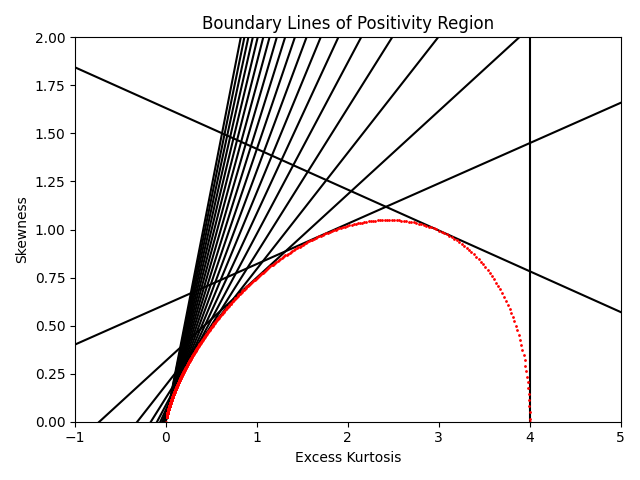
\includegraphics[width=0.4\textwidth]{img/gc_positivity_boundary_lines_20.png}
    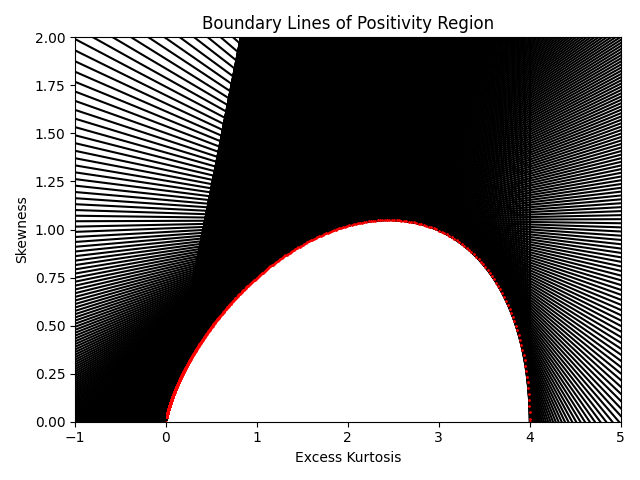
\includegraphics[width=0.4\textwidth]{img/gc_positivity_boundary_lines_1000.png}
    \caption{Boundary lines of the positivity region of the Gram-Charlier Expansion. The left image shows 20 lines, the right image shows 1000 lines. The red dots are the boundary points. The boundary is symmetric to the x-axis.}
    \label{fig:gram_charlier_boundary_lines_20_vs_1000}
\end{figure}

\begin{figure}[h]
    \centering
    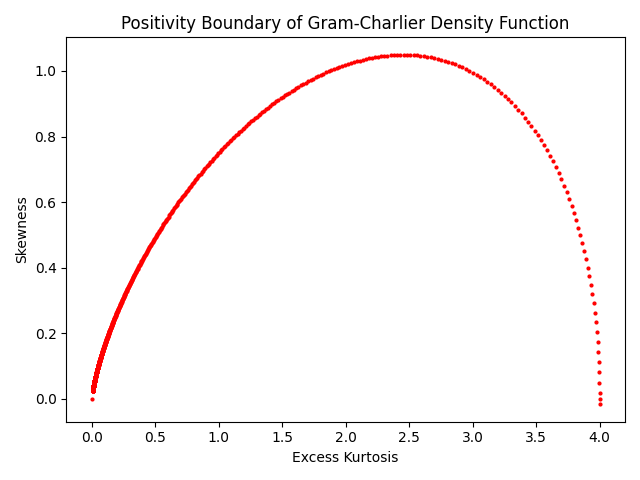
\includegraphics[width=0.8\textwidth]{img/gc_positivity_boundary.png}
    \caption{Approximation (1000 steps) of the positivity boundary of the Gram-Charlier Expansion. For simplicity, only the part above the x-axis is shown. The boundary is symmetric to the x-axis.}
    \label{fig:gram_charlier_boundary}
\end{figure}

- Using a bisection algorithm and a logisitc map, they make the boundary piecewise linear and find for each unconstraint pair $(\tilde{\gamma_1}, \tilde{\gamma_2^*})\in\mathbb{R}^2$ a constraint pair in the positivity region $(\gamma_1, \gamma_2^*)\in \mathcal{D}$.
- Finding a closed form expression for the boundary is difficult, even with 24 hours on a high performancce computer and Python's sympy library I was not able to find one.

\begin{table}[h]
    \centering
    \begin{tabular}{l|l|l|l|l|l|l|l|l}
        Distribution & Parameters & $\mu$ & $\sigma^2$ & $\kappa_3$ & $\gamma_1$ & $\kappa_4$ & $\gamma_2^*$ \\
        \hline
        Standardnormal & $\mu=0$, $\sigma=1$ & 0 & 1 & 0 & 0 & 0 & 0 \\
        Lognormal & $\mu=0$, $\sigma = 0.5$ & 1.1331 & 0.3647 & 0.3855 & 1.7502 & 0.7845 & 5.8984 \\
        t-Distribution & $\nu=5$ & 0 & 1.6667 & 0 & 0 & 16.6667 & 6 \\
        Non-Central t-Distribution & $\nu=5$, $\mu=0.5$ & 0.5947 & 1.7297 & 1.5357 & 0.6751 & 21.5969 & 7.2189
    \end{tabular}
    \caption{Distribution parameters and theoretical moments and cumulants.}
    \label{table:distributions_theoretical_moments}
\end{table}

\begin{figure}[h]
    \centering
    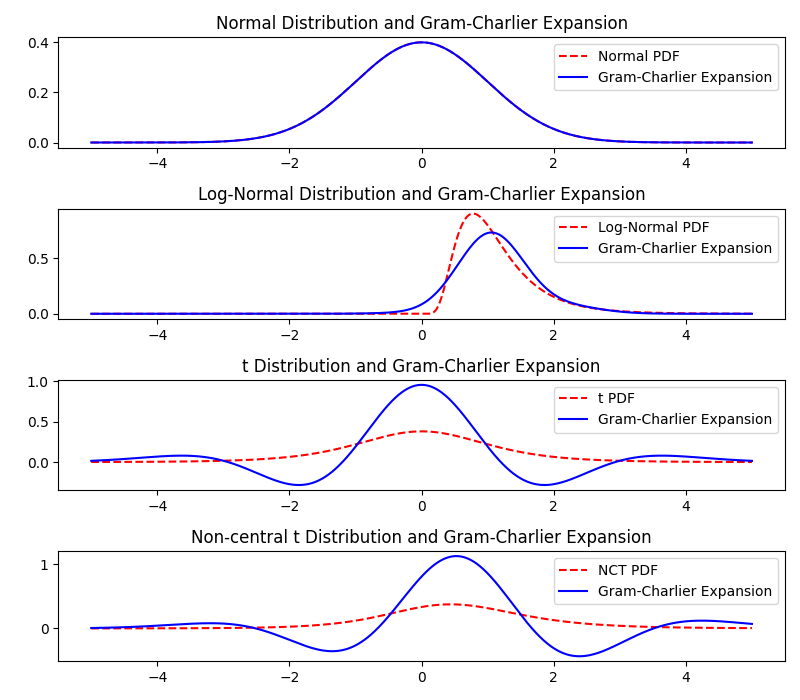
\includegraphics[width=0.8\textwidth]{img/gc_expansion.png}
    \caption{Gram-Charlier Expansion of different distributions}
    \label{fig:gc_expansion}
\end{figure}

\begin{figure}[h]
    \centering
    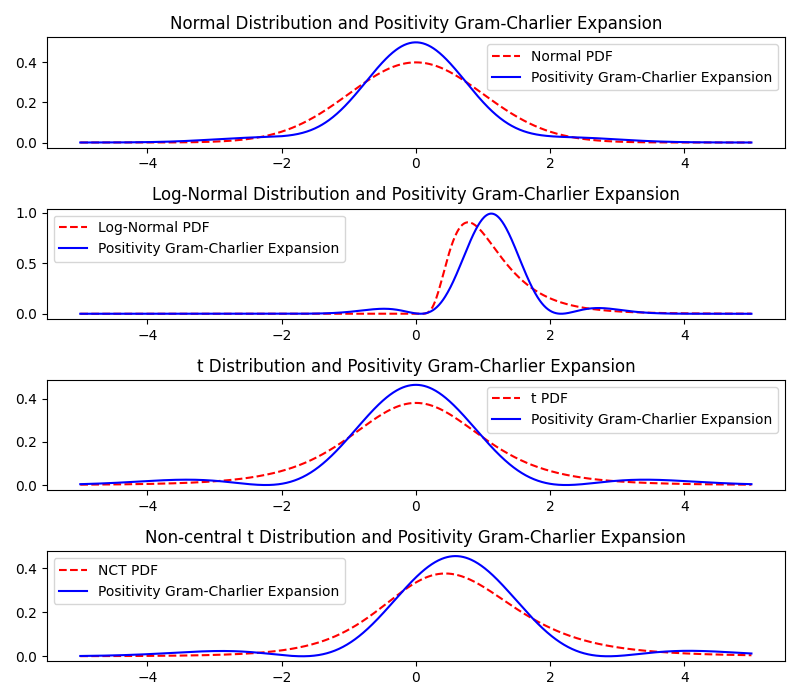
\includegraphics[width=0.8\textwidth]{img/gc_positivity_expansion.png}
    \caption{Gram-Charlier Expansion with positivity constraints of different distributions}
    \label{fig:gc_positivity_expansion}
\end{figure}

- Vergleich von constraint und unconstraint Parametern und dem Einfluss auf die Gram-Charlier Expansion. Test von 4 Verteilungen: Standardnormal, lognormal, t-Verteilung und Non-Central-T-Verteilung. Die Parameter und daraus resultierenden theoretischen Momente und Cumulants sind in Tabelle \ref{table:distributions_theoretical_moments} angegeben. Die Ergebnisse sind in Abbildung \ref{fig:gc_expansion} und Abbildung \ref{fig:gc_positivity_expansion} dargestelt. Man sieht sehr deutlich dass die positivity constraints notwendig sind, diese aber auch die Expansion verzerren, auch wenn, wie bei der Standardnormalverteilung, keine constraints notwendig gewesen wären. insbesondere hier wird durch die logisitic map eine Excess Kurtosis von 0 auf den Wert 2 gebracht, sodass das unconstrainte Paar $(\tilde{\gamma_1}, \tilde{\gamma_2^*}) = (0,0)$ zum constrainten Paar $(\gamma_1, \gamma_2^*) = (0,2)$ wird.

\subsection{Edgeworth Expansion}
- beschrieben von Edgeworth 1907, er schlägt unter anderem vor, die Approximation bis zum 6. Term zu berechnen um das oben angesprochene Problem der asympotischen Expansion zu umgehen. Eine formelle Darstellung der ersten Terme findet sich z.B. in Brenn & Anfinsen (2017):
\begin{align}
    f(x)_{EW} \approx \frac{1}{\sqrt{2\pi}\sigma}\exp\left(-\frac{(x-\mu)^2}{2\sigma^2}\right) \left[1 + \frac{\kappa_3}{6\sigma^3}H_3\left(\frac{x-\mu}{\sigma}\right) + \frac{\kappa_4}{24\sigma^4}H_4\left(\frac{x-\mu}{\sigma}\right) + \frac{\kappa_5}{120\sigma^5}H_5\left(\frac{x-\mu}{\sigma}\right) + \frac{\kappa_6 + 10\kappa_3^2}{720\sigma^6}H_6\left(\frac{x-\mu}{\sigma}\right)\right] \notag
\end{align}
In dieser Arbeit nur Betrachtung der ersten 4 Cumulants, daher reduziert sich der Ausdruck auf:
\begin{align}
    \label{eq:ew_expansion_short}
    f(x)_{EW} \approx \frac{1}{\sqrt{2\pi}\sigma}\exp\left(-\frac{(x-\mu)^2}{2\sigma^2}\right) \left[1 + \frac{\kappa_3}{6\sigma^3}H_3\left(\frac{x-\mu}{\sigma}\right) + \frac{\kappa_4}{24\sigma^4}H_4\left(\frac{x-\mu}{\sigma}\right) + \frac{\kappa_3^2}{72\sigma^6}H_6\left(\frac{x-\mu}{\sigma}\right)\right]
\end{align}
- Using same method as Jondeau & Rockinger (2001) to find the positivity boundary of the Edgeworth Expansion, we have to rewrite \eqref{eq:ew_expansion_short} with $z = \frac{x-\mu}{\sigma}$:
\begin{align}
    \label{eq:ew_expansion_s_ek}
    f(x)_{GC,A} \approx \frac{1}{\sqrt{2\pi}}\exp\left(-\frac{z^2}{2}\right) \left[1 + \frac{\gamma_1}{6}H_3(z) + \frac{\gamma_2^*}{24}H_4(z) + \frac{\gamma_1^2}{72}He_6(z)\right]
\end{align}
And then solve the equation $1 + \frac{\gamma_1}{6}He_3(z) + \frac{\gamma_2^*}{24}He_4(z) + \frac{\gamma_1^2}{72}He_6(z)=0$ for $\gamma_1$:
\begin{align}
    0 &= 1+\frac{\gamma_1}{6}He_3(z) + \frac{\gamma_2^*}{24}He_4(z) + \frac{\gamma_1^2}{72}He_6(z) \\
    0 &= \frac{72}{He_6(z)} + 12\gamma_1\frac{He_3(z)}{He_6(z)} + 3\gamma_2^*\frac{He_4(z)}{He_6(z)} + \gamma_1^2 \notag \\
    -\frac{72}{He_6(z)} - 3\gamma_2^*\frac{He_4(z)}{He_6(z)} &=  12\gamma_1\frac{He_3(z)}{He_6(z)} + \gamma_1^2 \notag \\
    -\frac{72}{He_6(z)} - 3\gamma_2^*\frac{He_4(z)}{He_6(z)} + 36\frac{He_3(z)^2}{He_6(z)^2} &= 12\gamma_1\frac{He_3(z)}{He_6(z)} + \gamma_1^2 + 36\frac{He_3(z)^2}{He_6(z)^2} \notag \\
    -\frac{72}{He_6(z)} - 3\gamma_2^*\frac{He_4(z)}{He_6(z)} + 36\frac{He_3(z)^2}{He_6(z)^2} &= \left(\gamma_1+6\frac{He_3(z)}{He_6(z)}\right)^2 \notag \\
    \gamma_1 &= \pm\sqrt{-\frac{72}{He_6(z)} - 3\gamma_2^*\frac{He_4(z)}{He_6(z)} + 36\frac{He_3(z)^2}{He_6(z)^2}} - 6\frac{He_3(z)}{He_6(z)} \notag
\end{align} %TODO: drüberlesen, ob alle s durch gamma_1 und alle k durch gamma_2^* ersetzt wurden
This holds as longs as $He_6(z)\neq 0$ which has 6 solutions:
\begin{align}
    z_{1/2} &= \pm \sqrt{5-\frac{5^{2/3}\left(1+i\sqrt{3}\right)}{\sqrt[3]{2\left(2+i\sqrt{6}\right)}} - \frac{\left(1-i\sqrt{3}\right)\sqrt[3]{5\left(2+i\sqrt{6}\right)}}{2^{2/3}}} = \pm 0.6167 \notag\\
    z_{3/4} &= \pm \sqrt{5-\frac{5^{2/3}\left(1-i\sqrt{3}\right)}{\sqrt[3]{2\left(2+i\sqrt{6}\right)}} - \frac{\left(1+i\sqrt{3}\right)\sqrt[3]{5\left(2+i\sqrt{6}\right)}}{2^{2/3}}} = \pm 1.8892 \notag \\
    z_{5/6} &= \pm \sqrt{5+\frac{10^{2/3}}{\sqrt[3]{2+i\sqrt{6}}} + \sqrt[3]{10\left(2+i\sqrt{6}\right)}} = \pm 3.3243 \notag
\end{align}

\begin{figure}[h]
    \centering
    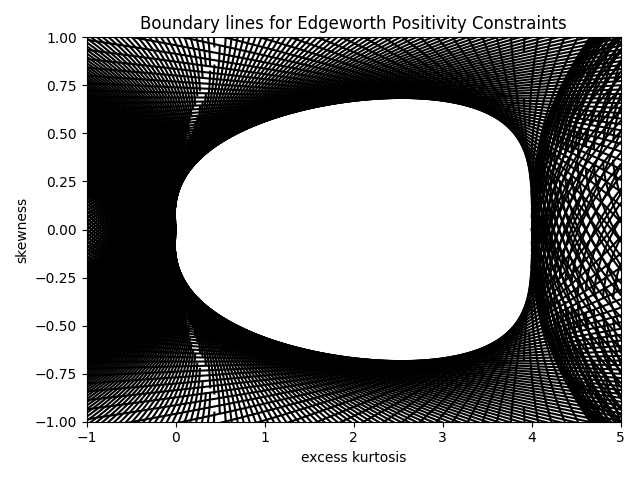
\includegraphics[width=0.8\textwidth]{img/edgeworth_positivity_boundary_lines.png}
    \caption{Boundary Lines for Edgeworth Expansion}
    \label{fig:ew_boundary_lines}
\end{figure}
\begin{figure}[h]
    \centering
    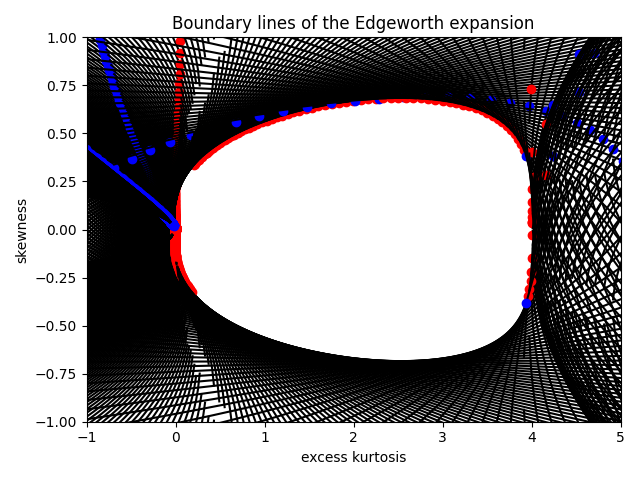
\includegraphics[width=0.8\textwidth]{img/edgeworth_positivity_boundary_intersections_1.png}
    \caption{Intersections of Boundary Lines for Edgeworth Expansion, red is first intersection, blue is second intersection}
    \label{fig:ew_boundary_intersections_1}
\end{figure}
\begin{figure}[h]
    \centering
    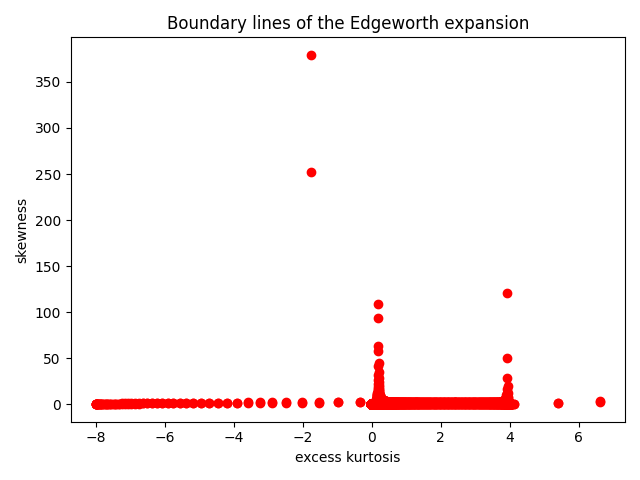
\includegraphics[width=0.8\textwidth]{img/edgeworth_positivity_boundary_intersections_3.png}
    \caption{Intersections of Boundary Lines for Edgeworth Expansion (zoomed out), upper half}
    \label{fig:ew_boundary_intersections_3}
\end{figure}
\begin{figure}[h]
    \centering
    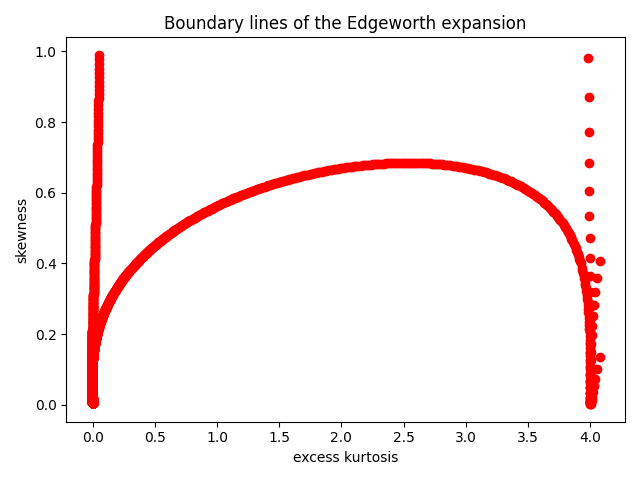
\includegraphics[width=0.8\textwidth]{img/edgeworth_positivity_boundary_intersections_4.png}
    \caption{Intersections of Boundary Lines for Edgeworth Expansion (zoomed in), upper half}
    \label{fig:ew_boundary_intersections_4}
\end{figure}
\begin{figure}[h]
    \centering
    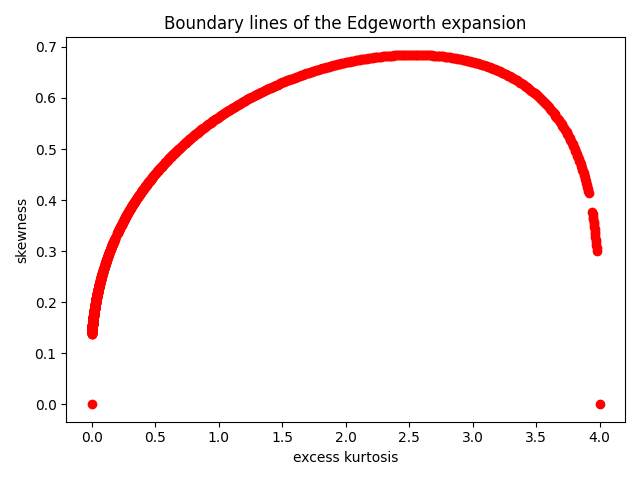
\includegraphics[width=0.8\textwidth]{img/edgeworth_positivity_boundary_intersections_7.png}
    \caption{Final Boundary Points for Edgeworth Expansion, upper half}
    \label{fig:ew_boundary_intersections_7}
\end{figure}

- Plot the lines $\gamma_1(\gamma_2^*, z)$ for many values of $z$ and skipping over the 6 singularities, we get \ref{fig:ew_boundary_lines}, much smaller than the GC boundary, for $\gamma_1 = 0$ excess kurtosis can be between 0 and 4. This is the same as for Gram-Charlier boundary because when skewness is 0, Gram-Charlier and Edgeworth expansion are the same. As for Gram-Charlier expansion, the boundary is the envelope of the lines $\gamma_1(\gamma_2^*, z)$, we get it by calculating the intersection of the two parabolas $\gamma_1(\gamma_2^*, z)$ and $\gamma_1(\gamma_2^*, z+\Delta z)$. These lines are parabolas and have the form $\gamma_1 = \sqrt{a(z) + b(z)\cdot \gamma_2^*} + c(z)$. For two different $z$, the parabolas $\gamma_{1,1} = \sqrt{a+b\gamma_2^*}+c$ and $\gamma_{1,2}=\sqrt{d+e\gamma_2^*}+f$ have the two intersections
\begin{align}
    \gamma_{2,1}^* &= \frac{2(b - e)^2(-c + f)\sqrt{-ab e + ae^2 + b^2 d + b c^2 e - 2 b c ef - bd e + b e f^2} + (b^2 - 2be + e^2)(-ab + ae + bc^2 - 2bcf + bd + bf^2 + c^2e - 2cef - de + ef^2)}{(b - e)^2(b^2 - 2be + e^2)} \notag \\
    \gamma_{1,1} &= c + \sqrt{a + b \cdot \left(\frac{2(b - e)^2(-c + f)\sqrt{-ab e + ae^2 + b^2 d + b c^2 e - 2 b c ef - bd e + b e f^2} + (b^2 - 2be + e^2)(-ab + ae + bc^2 - 2bcf + bd + bf^2 + c^2e - 2cef - de + ef^2)}{(b - e)^2(b^2 - 2be + e^2)}\right)} \notag \\
    \gamma_{2,2}^* &= \frac{2(b - e)^2(c - f)\sqrt{-ab e + ae^2 + b^2 d + b c^2 e - 2 b c ef - bd e + b e f^2} + (b^2 - 2be + e^2)(-ab + ae + bc^2 - 2bcf + bd + bf^2 + c^2e - 2cef - de + ef^2)}{(b - e)^2(b^2 - 2be + e^2)} \notag \\
    \gamma_{1,2} &= c + \sqrt{a + b \cdot \left(\frac{2(b - e)^2(c - f)\sqrt{-ab e + ae^2 + b^2 d + b c^2 e - 2 b c ef - bd e + b e f^2} + (b^2 - 2be + e^2)(-ab + ae + bc^2 - 2bcf + bd + bf^2 + c^2e - 2cef - de + ef^2)}{(b - e)^2(b^2 - 2be + e^2)}\right)} \notag
\end{align}
- For a plot of intersections (red dot is intersection 1, blue is intersection 2), see \ref{fig:ew_boundary_intersections_1}. Weil es immer zwei Schnittpunkte gibt, funktioniert die Methode von Jondeau & Rockinger (2001) nicht so gut. Daher Durchführung folgender Schritte, um die Positivitätsregion zu finden:
\begin{enumerate}
    \item boundary gets described mostly by red dots, so ignore second intersection. The envelope is symmetric around the $x$-axis and since we have for the boundary lines a second solution of the form $\gamma_1=-\sqrt{a(z)+b(z)\cdot \gamma_2^*}+c(z)$ which have the same intersection $\gamma_2^*$ and $-\gamma_1$, we can take the absolute of $\gamma_1$ for the red intersections and later mirror it around the $x$-axis.
    \item If we zoom out, we see many more intersection points which are not part of the boundary (\ref{fig:ew_boundary_intersections_3}). We know from the previous images that $\gamma_2^*$ is somewhat between 0 and 4 and $\gamma_1$ between -1 and 1, so we restrict the intersection points to have $\gamma_2^*\in (-0.1,4.1)$ and $\vert \gamma_1\vert \in [0,1)$ (\ref{fig:ew_boundary_intersections_4})
    \item The amount of points around $\gamma_2^*=0$ and going up too $\gamma_1=1$ are from intersections from boundary lines where $z$ is smaller than the negative third singularity, so leaving this out. The points around $\gamma_2^*=4$ are hard to filter out, they come from $\vert z\vert$ around 1.8 and 1.67 and I filtered them out by removing all $z$ where $z\in (1.8-0.035, 1.8+0.035)$ or $z\in (1.67-0.015,1.67+0.015)$
    \item I noticed that the boundary lines are extremly steep at this points, almost vertical and I get rounding errors, even when I use Python's float datatype which maps to IEEE-754 double precision with 64 bits where 52 bits are used for the fraction which equals about 16 decimal digits (Python Docs, Leonardo.Z (2013)). In general I am worried about computational accuracy since some points are at $\gamma_2^*>4$, ie. one point is at $(\gamma_2^*, \gamma_1) = (4.01, 0.222)$, but if I try to solve the following equation for $z$:
    \begin{align}
        1 + \frac{0.222}{6}He_3(z) + \frac{4.01}{24}He_4(z) + \frac{0.222^2}{72}He_6(z)<0 \notag
    \end{align}
    I find a solution: $-1.84611<z<-1.75826$. If this point is inside the boundary, there should be no solution, the Edgeworth expansion gives a density, but this is not the case. So to be on the safe side, I remove every intersection point that has not $\gamma_2^*\in [0,4]$. This is a very conservative approach, but I want to be sure that I do not have any false positives.
    \item I added $(0,0)$ and $(4,0)$ to the boundary points, the next and second last bondary points are $(3.7795\cdot 10^{-6}, 0.1378)$ and $(3.9775, 0.3009)$. A linear interpolation between these points gives the boundary (\ref{fig:ew_boundary_intersections_7}).
\end{enumerate}

\begin{figure}[h]
    \centering
    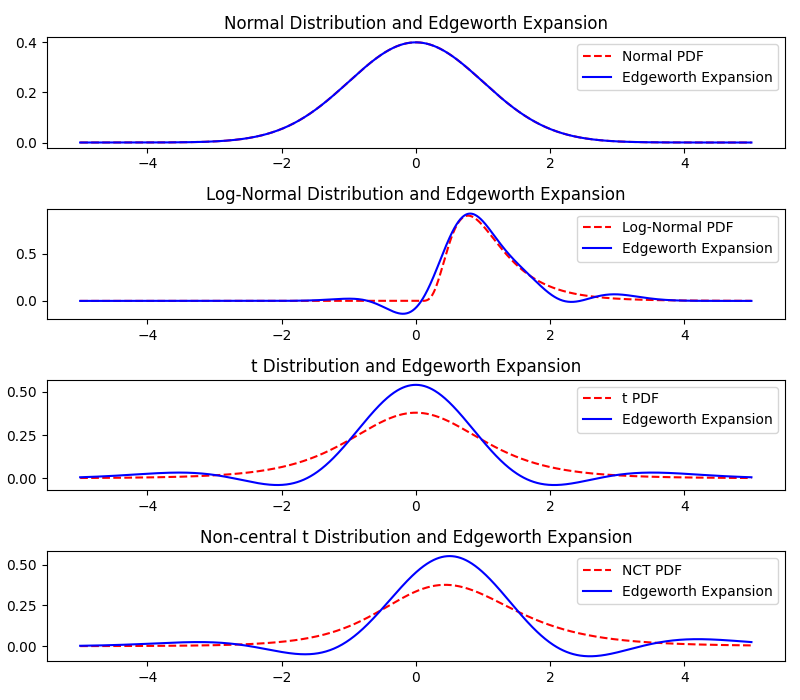
\includegraphics[width=0.8\textwidth]{img/ew_expansion.png}
    \caption{Edgeworth Expansion of different distributions}
    \label{fig:ew_expansion}
\end{figure}

\begin{figure}[h]
    \centering
    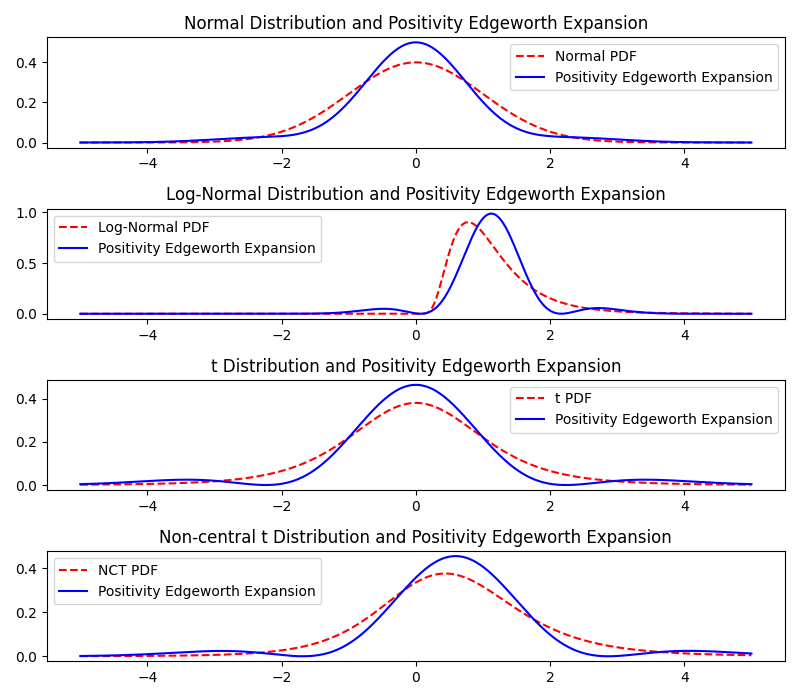
\includegraphics[width=0.8\textwidth]{img/ew_positivity_expansion.png}
    \caption{Edgeworth Expansion with positivity constraints of different distributions}
    \label{fig:ew_positivity_expansion}
\end{figure}

- Wir vergleichen wieder die constraint und unconstraint Parameter und den Einfluss auf die Edgeworth Expansion anhand der selben Verteilungen wie bei der Gram-Charlier Expansion (\ref{table:distributions_theoretical_moments}). Die Ergebnisse sind in Abbildung \ref{fig:ew_expansion} und Abbildung \ref{fig:ew_positivity_expansion} dargestelt. Die Schlussfolgerungen sind die selben wie bei der Gram Charlier Expansion: Man sieht sehr deutlich dass die positivity constraints notwendig sind, diese aber auch die Expansion verzerren, auch wenn, wie bei der Standardnormalverteilung, keine constraints notwendig gewesen wären.

\subsection{Cornish-Fisher Expansion}

\subsection{Saddlepoint Approximation}